\section{Application}
The main goal from the start has been to identify roads from Bing aerial maps.
To try this out an account with Bing maps API has been set up for educational
purposes. Two different locations were chosen as example areas to try the algorithm
on. The implementation used is the one created by Felzenszwalb and found on
his webpage at Brown University homepage \cite{web:sourceCode}. The additions
made to the algorithm is a wrapper with OpenCV library \cite{web:wrapper}.
The additions the wrapper gives is a GUI for faster testing of different
input values and the possibility to load any image type supported by OpenCV.

The first location is an aerial image over central parts of Lule\.{a} in northern
Sweden. The original is shown in figure \ref{fig:luleaOriginal} and the segmentation
is shown in figure \ref{fig:luleaEGBIS}.
\begin{figure}[ht]
    \begin{minipage}[t]{\linewidth}
        \centering
        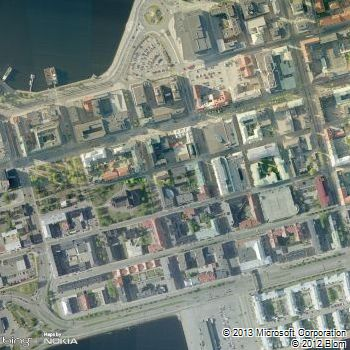
\includegraphics[width=\textwidth]{images/bing/lulea-original.jpg}
        \caption{Lule\.{a}, image from Bing Maps API}
        \label{fig:luleaOriginal}
    \end{minipage}
\end{figure}
The result from this segmentation presented here is one of the best. With other
values for input the segmentation becomes either to detailed or too rough
(too big regions).
\begin{figure}[ht]
    \begin{minipage}[t]{\linewidth}
        \centering
        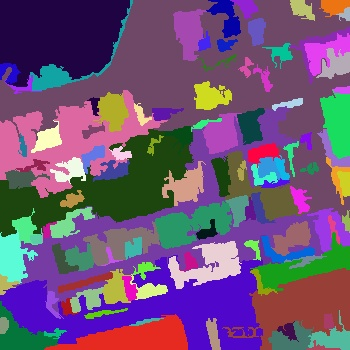
\includegraphics[width=\textwidth]{images/bing/lulea-egbis.jpg}
        \caption{Lule\.{a}, EGBIS segmentation, sigma at 0.8, k at 300 and c at 100}
        \label{fig:luleaEGBIS}
    \end{minipage}
\end{figure}

In figure \ref{fig:roadOriginal} a region with mostly forest, one highway passing
through in the middle and a few roads connecting to the highway at a junction is shown.
The segmentation from this is shown in figure \ref{fig:roadEGBIS}. The result shows
the highway clearly in the middle as a region but the smaller roads and the junction
is hard to identify unless you know that they exist.
\begin{figure}[ht]
    \begin{minipage}[t]{\linewidth}
        \centering
        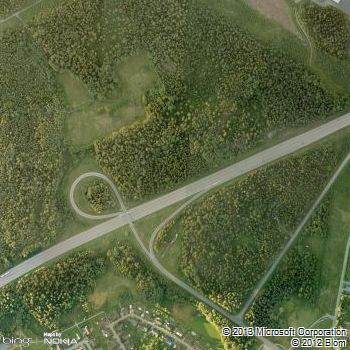
\includegraphics[width=\textwidth]{images/bing/road-original.jpg}
        \caption{Highway, image from Bing Maps API}
        \label{fig:roadOriginal}
    \end{minipage}
\end{figure}
\begin{figure}[ht]
    \begin{minipage}[t]{\linewidth}
        \centering
        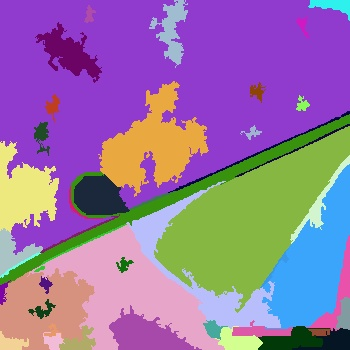
\includegraphics[width=\textwidth]{images/bing/road-egbis.jpg}
        \caption{Highway, EGBIS segmentation, sigma at 0.8, k at 300 and c at 100}
        \label{fig:roadEGBIS}
    \end{minipage}
\end{figure}
